\newpage
\section{Wstęp}
Rynek bezzałogowych statków powietrznych od kilku lat wykazuje niezwykle szybki rozwój. Cywilne BSP, coraz powszechniej nazywane po prostu ,,dronami'' także w urzędowych pismach, w roku 2018 osiągnęły wartość ok. 147~mln~zł \cite{bialaksiega2019}. Zwiększająca się liczba bezzałogowych operacji lotniczych i łatwość dostępu do sprzętu z tej dziedziny spowodowały między innymi aktualizację i ujednolicenie europejskich przepisów opisujących zasady wykonywania lotów \cite{eu-945-2019}.

\subsection{Motywacja}
W wyniku wprowadzenia nowych kategorii BSP oraz uprawnień dla operatorów, konieczna była zmiana programu szkolenia. Dużą zmianą jest wprowadzenie tzw. kategorii otwartej dla lotów o niskim ryzyku. Szkolenie do uzyskania tych uprawnień jest zrealizowane w formie komputerowej, korzystając z platformy online przygotowanej przez Urząd Lotnictwa Cywilnego \cite{ulc2019}. Wskazuje to, że można się spodziewać rosnącego udziału symulatorów w procesie szkolenia, podobnie jak ma to miejsce w przypadku komercyjnego lotnictwa załogowego.

Przed 31 grudnia 2020 roku, kiedy zostały wprowadzone nowe przepisy, szkolenie do wszystkich kategorii świadectwa kwalifikacji operatora bezzałogowego statku powietrznego (UAVO) odbywało się w formie tradycyjnej. Część teoretyczna w formie wykładów, po której następowały loty z instruktorem. Jedynym wskaźnikiem postępów kursanta, oraz kryterium zdania egzaminu praktycznego była opinia instruktora lub egzaminatora. Celem niniejszej pracy jest próba przygotowania symulatora BSP, który oprócz odwzorowania statku oferuje obiektywny wskaźnik jakości pilotażu pomocny w szkoleniu. Ocena prowadzona przez eksperta, niezależnie od poziomu jego doświadczenia, pozostaje subiektywna. Wprowadzenie dodatkowego narzędzia oferuje typowe zalety obiektywnych przyrządów pomiarowych jak większą powtarzalność, lub możliwość porównania wyników zebranych w różnych miejscach i ośrodkach szkoleniowych. Dodatkową zaletą jest poprawa procesu samodzielnego szkolenia ucznia. W pracy nie jest proponowane pełne zastąpienie instruktora w prowadzeniu szkolenia, ale możliwe że dzięki wykorzystaniu automatycznej oceny średniozaawansowany uczeń będzie mógł sam pracować nad swoimi umiejętnościami które wymagają najwięcej poprawy.

\subsection{Symulatory lotu}
Symulacją nazywa się imitację działania rzeczywistego procesu lub układu w czasie \cite{banks2010}. Etymologia tego słowa od łac.~\emph{simulātiō} słusznie wskazuje na wbudowany w symulację pewien fałsz czy oszustwo. Symulowanie rzeczywistości zawsze wymaga utworzenia modelu, który ma za zadanie reprezentować najważniejsze charakterystyki lub zachowania wybranego obiektu. W ścisłym znaczeniu, nie jako dziedzina nauki, symulacja to ewolucja stanu modelu w czasie \cite{banks2010}.

Symulacja może być wykorzystywana w różnych kontekstach, jednym z przykładów może być symulacja konkretnych technologii na etapie projektowania i produkcji, w celu poprawy własności. W pewnych dziedzinach nauki, tworzenie coraz lepszych modeli których symulowanie daje wyniki bardziej zbliżone do rzeczywistych procesów jest użytecznym narzędziem w celu zrozumienia tych zjawisk. Może być wykorzystywana kiedy praca na rzeczywistym obiekcie nie jest możliwa, ponieważ jest np. fizycznie niedostępny, niebezpieczny, jeszcze nie został zbudowany, lub takie postępowanie jest wysoce nieopłacalne ekonomicznie.

Z tych powodów, symulacja jest narzędziem szczególnie chętnie wykorzystywanym w lotnictwie \cite{neal2020}. Wykorzystanie symulatorów lotu pozwala ćwiczyć niebezpieczne manewry i sytuacje, mimo że pilot i instruktor znajdują się na ziemi bez zagrożenia dla nich lub statku powietrznego. Kolejną korzyścią jest zwiększenie intensywności treningu danego zadania. Przykładowo, ćwicząc lądowania w symulatorze, nie trzeba spędzać czasu wykonując także starty i podejścia. Ponadto, eksploatacja symulatora jest z reguły znacznie tańsza niż statku powietrznego w przeliczeniu na godzinę ćwiczeń. Mniejsza liczba rzeczywistych lotów szkoleniowych oprócz korzyści finansowych, powoduje także zmniejszenie ilości hałasu oraz emisji spalin, które składają się na negatywny wpływ lotnictwa na środowisko \cite{eaer2019}. Biorąc pod uwagę że każda flota statków powietrznych jest ograniczona do pewnej ich liczby, można zauważyć kolejną korzyść. Zmniejszona liczba szkoleniowych operacji lotniczych powoduje że większa część posiadanych zasobów sprzętowych i personalnych może być przeznaczona do wykonywania głównego celu działania danej organizacji.

Można wprowadzić różny podział symulatorów lotu ze względu na szczegóły ich działania: symulatory jednolite lub rozproszone, z modelami ciągłymi lub dyskretnymi. Jednak bardziej użyteczny wydaje się podział ze względu na przeznaczenie \cite{szczepanski1990}:
\begin{itemize}
  \item symulatory badawcze,
  \item symulatory szkoleniowe:
  \begin{itemize}
    \item symulatory ćwiczebne typu samolotów (nieruchome),
    \item rozbudowane symulatory samolotów (ruchome),
    \item symulatory walki powietrznej.
  \end{itemize}
\end{itemize}

Ponieważ wyszkolenie załogi ma duży wpływ na bezpieczeństwo operacji lotniczych, także symulatory lotnicze są uregulowane odpowiednimi przepisami. Szczegółowa klasyfikacja wprowadzona przez europejską agencję bezpieczeństwa lotnictwa (EASA), wygląda następująco \cite{cs-fstd}:
\begin{itemize}
  \item[FSTD] \emph{Flight simulator training device:}
  \begin{itemize}
    \item[FFS] \emph{Full flight simulator} -- pełnowymiarowa replika kokpitu konkretnego typu statku powietrznego wraz z wyposażeniem i oprogramowaniem niezbędnym do reprezentacji działania statku powietrznego w powietrzu i na ziemi, systemem wizualnym prezentującym widok z kokpitu, systemem symulującym odpowiednie siły na sterownicach (\emph{force cueing})
    \item[FTD] \emph{Flight training device} -- pełnowymiarowa replika kokpitu konkretnego statku powietrznego wraz z wyposażeniem i oprogramowaniem niezbędnym do reprezentacji działania statku powietrznego w powietrzu i na ziemi jedynie w zakresie systemów zainstalowanych w urządzeniu; nie są wymagane system wizualny ani sił na sterownicach
    \item[FNPT] \emph{Flight and Navigation procedure trainer} -- urządzenie treningowe reprezentujące środowisko kokpitu konkretnego typu lub klasy statków powietrznych wraz z wyposażeniem i oprogramowaniem niezbędnym do reprezentacji działania zainstalowanych systemów tak jakby były w statku powietrznym
    \item[BITD] \emph{Basic instrument training device} -- naziemne urządzenie szkoleniowe reprezentujące stanowisko pilota na klasie samolotów; może wyświetlać przyrządy za pomocą ekranów i używać sprężynowych sterownic, zapewniając jedynie podstawę do ćwiczenia proceduralnych aspektów lotu według przyrządów; dotyczy tylko samolotów, nie dotyczy śmigłowców
  \end{itemize} 
  \item[OTD] \emph{Other training device} -- pomoc szkoleniowa inna niż FSTD która może być używana do ćwiczeń gdzie nie jest niezbędne pełne środowisko kokpitu
\end{itemize}

Gdyby wykorzystać definicję FFS w kontekście symulacji bezzałogowego statku powietrznego, wymogi związane ze środowiskiem i układem sterowania są stosunkowo proste do spełnienia. Stosując nadajnik zdalnego sterowania, oraz oprogramowanie stacji naziemnej i układu automatycznego sterowania identyczne z tymi wykorzystywanymi w normalnym locie, operator obsługuje wszystkie systemy tak jak w normalnym locie. Większym problemem pozostaje kwestia modelowania dynamiki konkretnego BSP, oraz system wizualny. Ponieważ operator w przypadku lotów w zasięgu wzroku ma niemal nieograniczone pole widzenia, może być użyteczne zastosowanie wizualizacji immersyjnych, popularnie wykorzystywanych w celach rozrywkowych.

\subsection{Technologie gier komputerowych}
Podobnie jak inne rodzaje oprogramowania, gry komputerowe w ciągu ostatnich kilkudziesięciu lat od ich powstania przeszły wiele zmian. Stały się bardziej złożone, zawierają wizualizacje o większym stopniu skomplikowania, oraz co roku jest ich wydawane więcej. Ponieważ wiele gier zawiera te same elementy jak m.~in. wizualizacja, symulacja fizyki, zapisywanie i odczyt stanu z pamięci, lub obsługa dźwięku, wymagają rozwiązania podobnych problemów inżynieryjnych. Obecnie niemal wszystkie gry korzystają z jakiejś formy tzw. ,,silnika gry'', czyli podstawowego oprogramowania koniecznego do jej działania. Sam silnik nie jest grą, tylko bardziej podstawowym narzędziem; platformą w której łączony jest kod, zasoby multimedialne\footnote{ang. \emph{assets}} oraz inne dane żeby wyprodukować grę \cite{toftedahl2019}.

Tradycyjnie, techniki renderowania czyli komputerowego wytwarzania obrazu różniły się znacząco dla gier oraz innych mediów. W przeciwieństwie do symulatora lub gry, obliczenia wykonywane w celu wytworzenia jednego obrazu lub kolejnych klatek filmu mogą trwać dłużej niż niewielka część sekundy. Jednak stały rozwój narzędzi, sprzętu komputerowego oraz coraz lepszych technik programowania sprawiły, że od niedawna jest możliwe generowanie obrazów o bardzo wysokim stopniu realizmu w czasie rzeczywistym. Dzięki temu, silniki gier wykorzystywane są w nowych dziedzinach, poprzednio zarezerwowanych dla dedykowanego oprogramowania. Przykładowo, w przemyśle motoryzacyjnym utworzono w ten sposób wizualizację zamawianego samochodu, która przedstawia właśnie wybieraną konfigurację \cite{audi2021}. Także część niedawno wydanych filmów wykorzystuje silnik gry do przygotowywania efektów specjalnych lub teł dla aktorów \cite{nfs2020}.

Poza oprogramowaniem do renderowania, także wyświetlacze przeszły duże zmiany. W 2012 roku na targach E3 zaprezentowano urządzenie Oculus Rift, będące pierwszym HMD\footnote{\emph{Head-Mounted Display}} skierowanym do konsumentów \cite{rubin2014}. Wyświetlany obraz zależny od położenia głowy, tworzy iluzję bycia otoczonym ze wszystkich stron przez generowany przez komputer widok, stąd termin rzeczywistość wirtualna (VR). Na rysunku \ref{fig:badania-vr} przedstawiono zdjęcie z wykonywanych testów systemu, na którym wykorzystywane są okulary VR. Poprzednio urządzenia tego typu były wykorzystywane tylko w placówkach naukowych lub wojskowych. Od tamtej pory na rynku pojawiły się urządzenia od różnych producentów. W kolejnych latach poprawiano czas reakcji wyświetlacza, rozdzielczość, pole widzenia, techniki śledzenia okularów i kontrolerów.

\begin{figure}[!h]
    \centering 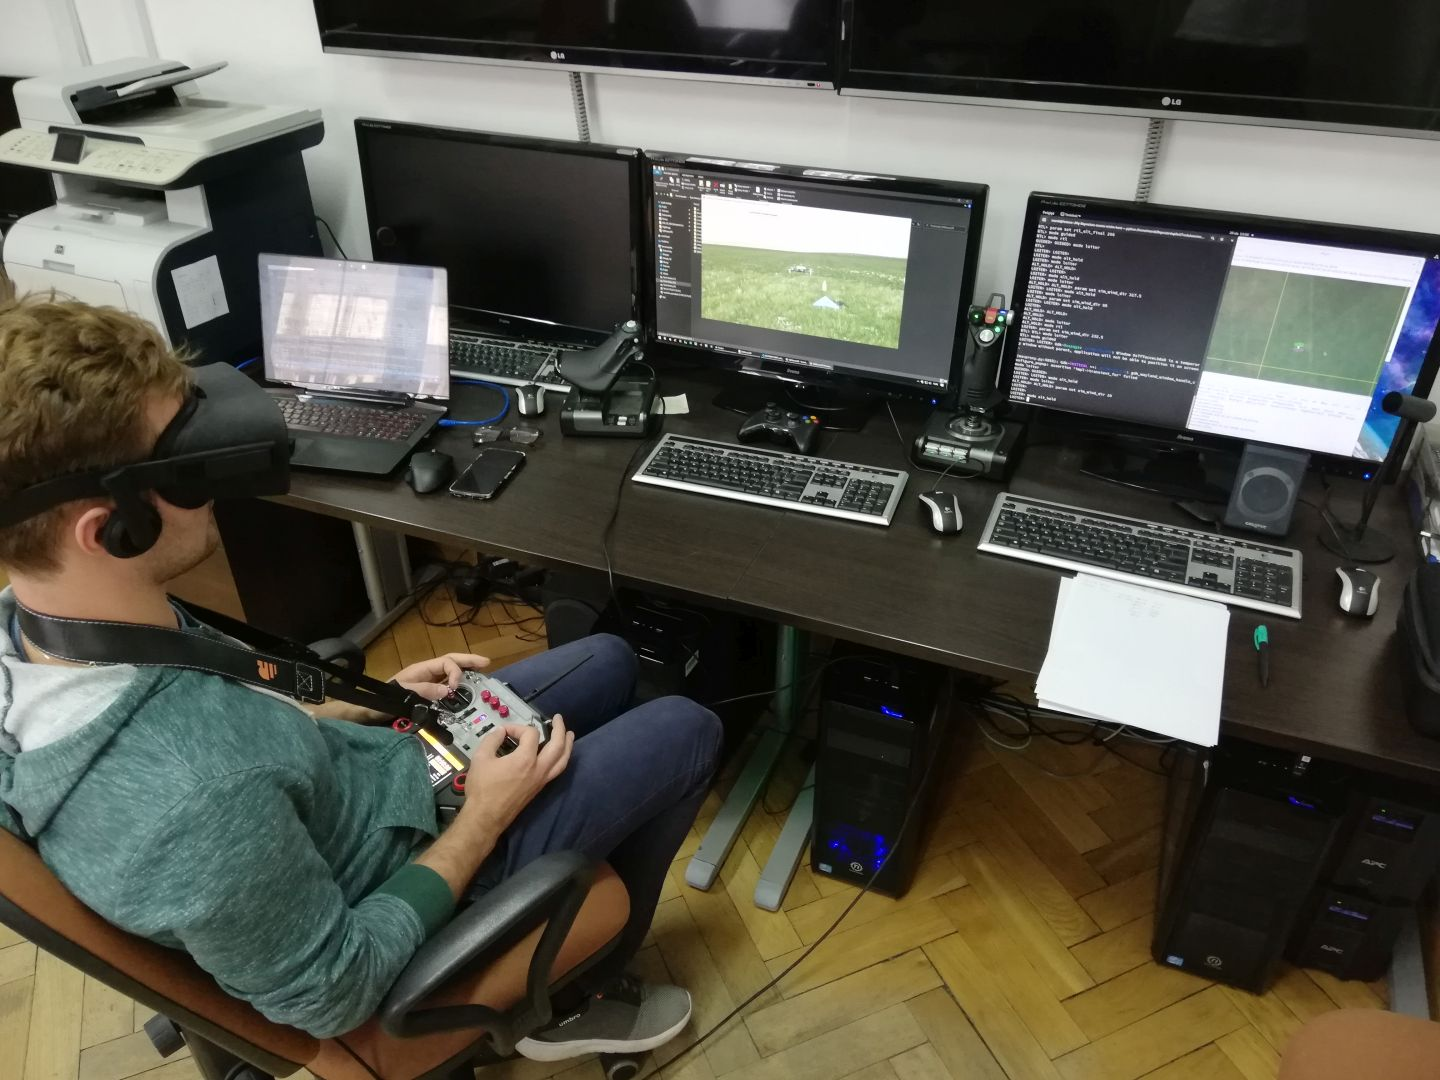
\includegraphics[width=0.8\linewidth]{badania-vr.jpg}
    \caption{Operator BSP obserwujący symulację przez wyświetlacz Oculus Rift}
    \label{fig:badania-vr}
\end{figure}

Możliwość zajęcia całego pola widzenia symulowanym obrazem, oraz śledzenie ruchów rąk sprawiają że HMD także są wykorzystywane nie tylko w grach komputerowych. Ponieważ jeszcze nie ma popularnych rozwiązań stymulujących zmysł dotyku, trening w wirtualnej rzeczywistości często dotyczy prowadzenia pojazdów, lub nauki wykonywania odpowiednich procedur. Przykładowym zastosowaniem może być szkolenie operatorów maszyn budowlanych \cite{cmlabs2021}, albo demontażu złożonego silnika lotniczego \cite{inlusion2020}. Ważnym przełomem jest certyfikacja przez EASA pierwszego urządzenia treningowego wykorzystującego okulary VR \cite{easavr2021}. Jest to symulator typu FNPT dla śmigłowca Robinson R22.

\subsection{Dostępne rozwiązania}
Duża liczba spośród obecnie oferowanych symulatorów BSP jest skierowana do osób zainteresowanych zdalnie sterowanymi modelami latającymi. To przeznaczenie powoduje że ich użyteczność w szkoleniu UAVO jest bardzo ograniczona. Spośród dostępnego oprogramowania w tej kategorii wyróżnia się RealFlight \cite{realflight}, który można połączyć z autopilotem oraz zawiera modele różnych wielowirnikowców. Niestety otoczenie w którym wykonywany jest lot zawiera jedynie pas startowy i okazjonalnie inne przeszkody, natomiast szkolenie operatorów wymaga m.~in. wykonywania konkretnych manewrów w określonym miejscu. Alternatywą która jest przeznaczona do ćwiczenia zawodowych, a nie sportowych zadań jest DJI Flight Simulator \cite{djifs}. Zawiera kilka modeli wielowirnikowców, ale tylko wyprodukowanych przez DJI, poza tym jest kompletnym, zamkniętym systemem bez możliwości modyfikacji lub łączenia z innymi aplikacjami.

Symulatory lotu dla załogowych statków powietrznych mogłyby po modyfikacjach służyć jako podstawa do opracowania systemu. Wykorzystywany także w publikacjach naukowych X-Plane \cite{xplane} bywał łączony m.~in. z oprogramowaniem MATLAB, ale zawiera tylko samoloty i śmigłowce. Alternatywny FlightGear \cite{flightgear} ma otwarty kod źródłowy, a nawet zaimplementowane kilka modeli bezzałogowych statków powietrznych. Niestety wszystkie trzy z nich są samolotami, więc implementacja wielowirnikowca wiązałaby się prawdopodobnie z dużym nakładem pracy.

Ostatnią rozważaną grupą są symulatory przeznaczone dla rozwijania systemów robotyki. Niektóre z nich jak Gazebo \cite{gazebo} lub MorseSim mają gotowe modele dynamiczne wielowirnikowców, a także opracowane sposoby łączenia z autopilotem. Dostęp do kodu źródłowego oraz przeznaczenia badawcze sprawiają że są w wysokim stopniu konfigurowalne. Ich główną wadą jest przeznaczenie do symulowania otoczenia na potrzeby automatycznego systemu robota, a nie człowieka. Z tego powodu ich warstwa graficzna jest dość podstawowa, wystarczająca jedynie do nadzorowania przebiegu procesu. Wyjątkiem od tej charakterystyki jest AirSim \cite{airsim2017}. Głównym celem tego oprogramowania jest dostarczenie platformy do tworzenia sterowników wykorzystujących uczenie maszynowe. Ponieważ obraz z kamery w paśmie widzialnym jest jednym z czujników wykorzystywanych w tych systemach, twórcy zaimplementowali realistycznie wyglądającą grafikę.

Byłoby możliwe utworzenie systemu oceny w oparciu o AirSim, jednak wymagałoby to licznych modyfikacji do obsługi przez ludzi. Końcowy produkt prawdopodobnie miałby niezrozumiałe dla użytkownika cechy które wynikają z adaptacji oprogramowania przeznaczonego początkowo do innego celu. Zdecydowano że zamiast tego lepiej będzie wykorzystać surowy silnik gry i dodać do niego tylko wykorzystywane funkcje. Dzięki temu oczekiwany jest mniejszy, łatwiejszy w obsłudze i bardziej niezależny system.
